\documentclass[a4paper,12pt]{article}
\usepackage{czech}
\usepackage[utf8]{inputenc}
\usepackage{a4wide}
\usepackage[dvipdfm]{graphicx}
\usepackage{graphics}
\usepackage{indentfirst}
\usepackage{fancyhdr}
\usepackage{setspace}
\usepackage{amsmath}
\usepackage{amssymb}
\usepackage{epsfig}

%%\usepackage{nopageno}
%%\usepackage{txfonts}
\usepackage[usenames]{color}

\begin{document}
\section{Úkol}
\noindent
\begin{enumerate}
    \item Proměřte voltampérovu charakteristiku diaku a z ní určete:
    \begin{enumerate}
        \item spínací napětí při obou polaritách $U_{BO1},U_{BO2}$
        \item pokles napětí na diaku při překročení spínacího napětí $\Delta U$ (při obou polaritách)
        \item tzv. symetrii diaku $|U_{BO1}-U_{BO2}|$.
    \end{enumerate}
    \item Zapojte diak jako zdroj relaxačních kmitů a změřte závislost periody těchto kmitů $T$ na časové 
    kostantě $\tau = RC$ obvodu při konstantním napětí zdroje (cca 40 V). Kmitočet relaxačních kmitů měřte 
    běžně čítačem, při několika řádově různých hodnotách všah též přímo osciloskopem s porovnáním s kmitočtem 
    generátoru (pomocí Lissajousových obrazců). V referátu porovnejte přesnost použitých metod měření kmitočtů.
    \item Změřte závislost frekvence kmitů $f$ na napětí zdroje $U_O$. Pomocí osciloskopu určete z amplitud 
    relaxačních kmitů hodnoty zhášecích napětí $U_{zh}$ a naměřené hodnoty ověřte výpočtem.
\end{enumerate}

\section{Teorie}

\subsection{Diak}
    Diak je elektrická součástka tvořená třemi vrstvami polovodiče, na kterých jsou dvě elektrody. 
    Schéma je na obrázku 1 v \cite{text}. Jeho voltampérová charakteristika se vyznačuje tím, že 
    je nutné dosáhnout jistého spínacího napětí $U_{BO}$, aby ním začal protékat proud. Na této hranici 
    prudce klesne napětí o $\Delta U$ a proud se vyvijí dle obrázku 2 v \cite{text}. Při příliš malém 
    proudu se diak opět zavře a proud přestane téci úplně. VA charakteristika je symetrická, proto se 
    zavádí další charakteristika zvaná symetrie diaku, která je určena vztahem $|U_{BO1}-U_{BO2}|$, kde 
    jednotlivá napětí jsou zápalné napětí pro různé polarizace.

\subsection{Měření VA charakteristiky}
    Měříme v zapojení na obrázku 3 v \cite{text}. Odpor $R$ si nastavíme na hodnotu 5 k$\Omega$. Zvyšujeme napětí 
    na diaku, dokud nezačne téci proud. Díky maximálnímu voltmetru určíme $U_{BO}$. Dále měníme napětí od maximální 
    hodnoty, při které nesmíme překročit zrrátový výkon $P= 300$mW, až do bodu, kdy proud opět přestane téci. Opakujeme 
    pro obě polarizace.

\subsection{Relaxační kmity}
    Měření probíhá v zapojení dle obrázku 4 z \cite{text}. Paralelně k diaku je zapojen kondenzátor. Te se při uzavření obvodu 
    začne nabijet. Jakmile dosáhne napětí hodnoty $U_{BO}$, diak se sepne a kondenzátor se vybije. Napětí klesne až na hodnotu 
    zhášecího napětí $U_{zhs}$. Diak se opět uzavře. Celý cyklus začíná znocu. Teoretický průběh proudu je vidět na obrázku 5a z 
    \cite{text}. Frekvenci tohoto děje můžeme nejejdnodušeji odečíst z čítače. Dále můžeme využít osciloskop ke stanocení periody 
    kmitu nebo při zapojení druhého zdroje kmitů do osciloskopu můžeme dosáhnout Lissajousova obrazce, kdy se frekvence zdrojů 
    shodují, a tak ji můžeme odečíst z druhého zdroje.

    Teoretická doba jednoho kmitu je dle \cite{text}
    \begin{eqnarray}
    T=RC\cdot\ln\left(\frac{U_0-U_{zh}}{U_0-U_{BO}}\right).
    \label{T}
    \end{eqnarray}

\subsection{Chyby}
    V celém praktiku vystupují chyny způsobené nepřesnostní měřících přístrojů. Její velikost je dána třídou přesnosti měřidla.
    Její hodnotu získáme dle vztahu
    \begin{eqnarray}
    \sigma = T\cdot \frac{R}{100},
    \end{eqnarray}
    kde $T$ je třída přesnosti a $R$ rozsah, na kterém měříme.

    Dále vystupuje nepřímá chyba způobená skládáním chyb. V tomto praktiku se vystupuje pouze chyba rozdílu veličin, kdy se abosluní
    chyby sčítají, a podílu s násobkem, kdy se sčítají relativní chyby.


\section{Výsledky Měření}
\subsection{VA charakteristika}
    Dle postupu uvedeném v teorii jsem prověřil VA charakteristiku daného diaku. Zápalné napětí byla
    \begin{eqnarray}
        U_{BO1}=(32.8\pm0.2)\mbox{V}, \label{UBO1} \\
        U_{BO2}=(-32.7\pm0.2)\mbox{V}.
    \end{eqnarray}
    symetrie diaku je tedy
    \begin{eqnarray}
    |U_{BO1}-U_{BO2}|=(65.5 \pm 0.4)\mbox{V}.
    \end{eqnarray}
    Napětí kleslo o 
    \begin{eqnarray}
    \Delta U_1=(10.1 \pm 0.4)\mbox{V}, \\
    \Delta U_2=(9.9 \pm 0.4)\mbox{V}, \label{DU2}
    \end{eqnarray}
    Velikost proudu v průběhu vyšetřování je v tabulce \ref{TUk1}, kde chyba na napětí je 0.2 V, a výsledná charakteristika je na obrázku \ref{g1}.

    \begin{table}
    $$
    \begin{array}{|c|c||c|c|}
    \hline
    U/\mbox{V} & I/\mbox{mA} &  -U/\mbox{V} & -I/\mbox{mA} \\ \hline 
    22.9&   1.5 \pm 0.1&    23&  1.5\pm0.1 \\ \hline
    22.7&   2 \pm 0.1&  22.8&   2\pm 0.1 \\ \hline
    22.4&   3 \pm 0.1&  22.5&   3\pm0.1 \\ \hline
    22.3&   4 \pm 0.1&  22.3&   4\pm 0.1 \\ \hline
    22.1&   5 \pm 0.1&  22.1&   5\pm0.1 \\ \hline
    22.0&   6 \pm 0.1&  22.0&   6\pm0.1 \\ \hline
    21.9&   7 \pm 0.2& 21.9&   7\pm0.2 \\ \hline
    21.8&   8 \pm 0.2& 21.8&   8 \pm 0.2 \\ \hline
    21.7&   9 \pm 0.2& 21.7&   9 \pm 0.2 \\ \hline
    21.6&   10 \pm 0.2&21.6&   10 \pm 0.2 \\ \hline
    \end{array}
    $$
    \caption{Závislost proudu na napětí na diaku.}
    \label{TUk1}
    \end{table}
    
    \begin{figure}
    % GNUPLOT: LaTeX picture with Postscript
\begingroup
  \makeatletter
  \providecommand\color[2][]{%
    \GenericError{(gnuplot) \space\space\space\@spaces}{%
      Package color not loaded in conjunction with
      terminal option `colourtext'%
    }{See the gnuplot documentation for explanation.%
    }{Either use 'blacktext' in gnuplot or load the package
      color.sty in LaTeX.}%
    \renewcommand\color[2][]{}%
  }%
  \providecommand\includegraphics[2][]{%
    \GenericError{(gnuplot) \space\space\space\@spaces}{%
      Package graphicx or graphics not loaded%
    }{See the gnuplot documentation for explanation.%
    }{The gnuplot epslatex terminal needs graphicx.sty or graphics.sty.}%
    \renewcommand\includegraphics[2][]{}%
  }%
  \providecommand\rotatebox[2]{#2}%
  \@ifundefined{ifGPcolor}{%
    \newif\ifGPcolor
    \GPcolorfalse
  }{}%
  \@ifundefined{ifGPblacktext}{%
    \newif\ifGPblacktext
    \GPblacktexttrue
  }{}%
  % define a \g@addto@macro without @ in the name:
  \let\gplgaddtomacro\g@addto@macro
  % define empty templates for all commands taking text:
  \gdef\gplbacktext{}%
  \gdef\gplfronttext{}%
  \makeatother
  \ifGPblacktext
    % no textcolor at all
    \def\colorrgb#1{}%
    \def\colorgray#1{}%
  \else
    % gray or color?
    \ifGPcolor
      \def\colorrgb#1{\color[rgb]{#1}}%
      \def\colorgray#1{\color[gray]{#1}}%
      \expandafter\def\csname LTw\endcsname{\color{white}}%
      \expandafter\def\csname LTb\endcsname{\color{black}}%
      \expandafter\def\csname LTa\endcsname{\color{black}}%
      \expandafter\def\csname LT0\endcsname{\color[rgb]{1,0,0}}%
      \expandafter\def\csname LT1\endcsname{\color[rgb]{0,1,0}}%
      \expandafter\def\csname LT2\endcsname{\color[rgb]{0,0,1}}%
      \expandafter\def\csname LT3\endcsname{\color[rgb]{1,0,1}}%
      \expandafter\def\csname LT4\endcsname{\color[rgb]{0,1,1}}%
      \expandafter\def\csname LT5\endcsname{\color[rgb]{1,1,0}}%
      \expandafter\def\csname LT6\endcsname{\color[rgb]{0,0,0}}%
      \expandafter\def\csname LT7\endcsname{\color[rgb]{1,0.3,0}}%
      \expandafter\def\csname LT8\endcsname{\color[rgb]{0.5,0.5,0.5}}%
    \else
      % gray
      \def\colorrgb#1{\color{black}}%
      \def\colorgray#1{\color[gray]{#1}}%
      \expandafter\def\csname LTw\endcsname{\color{white}}%
      \expandafter\def\csname LTb\endcsname{\color{black}}%
      \expandafter\def\csname LTa\endcsname{\color{black}}%
      \expandafter\def\csname LT0\endcsname{\color{black}}%
      \expandafter\def\csname LT1\endcsname{\color{black}}%
      \expandafter\def\csname LT2\endcsname{\color{black}}%
      \expandafter\def\csname LT3\endcsname{\color{black}}%
      \expandafter\def\csname LT4\endcsname{\color{black}}%
      \expandafter\def\csname LT5\endcsname{\color{black}}%
      \expandafter\def\csname LT6\endcsname{\color{black}}%
      \expandafter\def\csname LT7\endcsname{\color{black}}%
      \expandafter\def\csname LT8\endcsname{\color{black}}%
    \fi
  \fi
  \setlength{\unitlength}{0.0500bp}%
  \begin{picture}(7200.00,5040.00)%
    \gplgaddtomacro\gplbacktext{%
      \csname LTb\endcsname%
      \put(1210,704){\makebox(0,0)[r]{\strut{} 500}}%
      \put(1210,1383){\makebox(0,0)[r]{\strut{} 600}}%
      \put(1210,2061){\makebox(0,0)[r]{\strut{} 700}}%
      \put(1210,2740){\makebox(0,0)[r]{\strut{} 800}}%
      \put(1210,3418){\makebox(0,0)[r]{\strut{} 900}}%
      \put(1210,4097){\makebox(0,0)[r]{\strut{} 1000}}%
      \put(1210,4775){\makebox(0,0)[r]{\strut{} 1100}}%
      \put(1342,484){\makebox(0,0){\strut{}-8}}%
      \put(2033,484){\makebox(0,0){\strut{}-6}}%
      \put(2724,484){\makebox(0,0){\strut{}-4}}%
      \put(3415,484){\makebox(0,0){\strut{}-2}}%
      \put(4106,484){\makebox(0,0){\strut{} 0}}%
      \put(4796,484){\makebox(0,0){\strut{} 2}}%
      \put(5487,484){\makebox(0,0){\strut{} 4}}%
      \put(6178,484){\makebox(0,0){\strut{} 6}}%
      \put(6869,484){\makebox(0,0){\strut{} 8}}%
      \put(308,2739){\rotatebox{-270}{\makebox(0,0){\strut{}$H$/Am$^{-1}$}}}%
      \put(4105,154){\makebox(0,0){\strut{}$x$/cm}}%
    }%
    \gplgaddtomacro\gplfronttext{%
      \csname LTb\endcsname%
      \put(5882,4602){\makebox(0,0)[r]{\strut{}12 cm}}%
      \csname LTb\endcsname%
      \put(5882,4382){\makebox(0,0)[r]{\strut{}16 cm}}%
      \csname LTb\endcsname%
      \put(5882,4162){\makebox(0,0)[r]{\strut{}20 cm}}%
    }%
    \gplbacktext
    \put(0,0){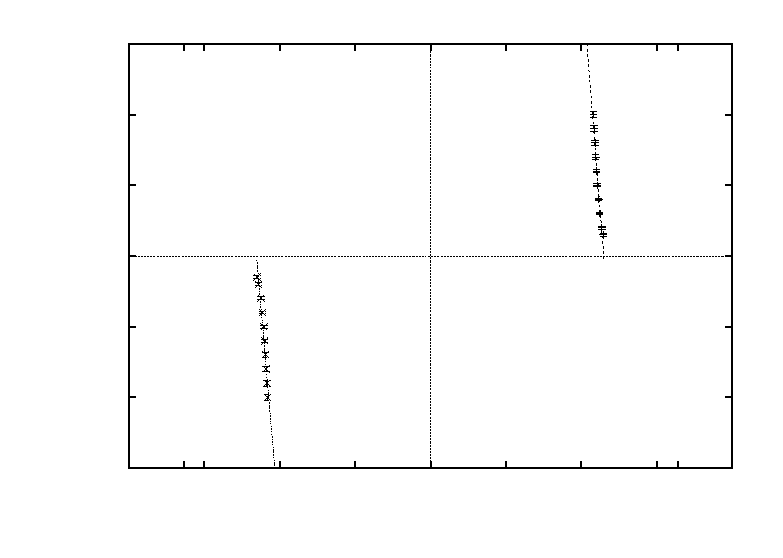
\includegraphics{g1}}%
    \gplfronttext
  \end{picture}%
\endgroup

    \caption{VA charakteristika diaku}
    \label{g1}
    \end{figure}

\subsection{Harmonické kmity}
    Dále jsem zapojel diak jako zdroj harmonických kmitů na na čítači měřil jejich frekvenci v závislosti na $\tau = RC$. Tyto hondoty jsou shrnuty 
    v tabulce \ref{TUk2} a zobrazeny na obrázku \ref{g2}. Pro tři řádově odlišné hodnoty frekvence jsem ještě použil jiné metody měření uvedené v teorii. 
    Tyto hodnoty jsou v tabulce \ref{TUk2b}, kde $f_o$ je hodnota vypočtená z periody kmitu určené osciloskopem, $f_{L1}$ respektive $f_{L2}$ hodnota stanovena pomocí Lissajousových 
    obrazců odečtená ze stupnice generátoru respektive z čítače napojeném za generátorem.
    
    \begin{table}
    $$
    \begin{array}{|c|c|}
    \hline
    \tau/\mbox{F}\Omega&    f/\mbox{Hz} \\ \hline
    250\pm1&    4920\pm50 \\ \hline
    300\pm1&    3600\pm40 \\ \hline
    350\pm1&    2980\pm30 \\ \hline
    400\pm1&    2510\pm30 \\ \hline
    450\pm1&    2150\pm20 \\ \hline
    500\pm1&    1890\pm20 \\ \hline
    1000\pm6&   714\pm7 \\ \hline
    1500\pm9&   438\pm4 \\ \hline
    2000\pm10&   315\pm3 \\ \hline
    2500\pm20&   279\pm3 \\ \hline
    3000\pm20&   225\pm2 \\ \hline
    3500\pm20&   188\pm2 \\ \hline
    4000\pm20&   162\pm2 \\ \hline
    4500\pm30&   143\pm1 \\ \hline
    5000\pm30&   128\pm1 \\ \hline
    \end{array}
    $$
    \caption{Závislost frekcence kmitů na časové konstantě $\tau$.}
    \label{TUk2}
    \end{table}

    \begin{table}
    $$
    \begin{array}{|c|c|c|c|}
    \hline
    \tau/\mbox{F}\Omega&    f_o/\mbox{Hz}&  f_{L1}/\mbox{Hz}& f_{L2}/\mbox{Hz} \\ \hline
    250\pm1&    4930\pm70&  4870\pm50&  4750\pm50 \\ \hline
    2500\pm20&  278\pm4&    271\pm5&    274\pm3 \\ \hline
    5000\pm30&  128\pm2&    129\pm1&    130\pm1 \\ \hline
    \end{array}
    $$
    \caption{Závislost frekvence kmitů na na $\tau$ měřená různými metodami.}
    \label{TUk2b}
    \end{table}
    
    \begin{figure}
    % GNUPLOT: LaTeX picture with Postscript
\begingroup
  \makeatletter
  \providecommand\color[2][]{%
    \GenericError{(gnuplot) \space\space\space\@spaces}{%
      Package color not loaded in conjunction with
      terminal option `colourtext'%
    }{See the gnuplot documentation for explanation.%
    }{Either use 'blacktext' in gnuplot or load the package
      color.sty in LaTeX.}%
    \renewcommand\color[2][]{}%
  }%
  \providecommand\includegraphics[2][]{%
    \GenericError{(gnuplot) \space\space\space\@spaces}{%
      Package graphicx or graphics not loaded%
    }{See the gnuplot documentation for explanation.%
    }{The gnuplot epslatex terminal needs graphicx.sty or graphics.sty.}%
    \renewcommand\includegraphics[2][]{}%
  }%
  \providecommand\rotatebox[2]{#2}%
  \@ifundefined{ifGPcolor}{%
    \newif\ifGPcolor
    \GPcolorfalse
  }{}%
  \@ifundefined{ifGPblacktext}{%
    \newif\ifGPblacktext
    \GPblacktexttrue
  }{}%
  % define a \g@addto@macro without @ in the name:
  \let\gplgaddtomacro\g@addto@macro
  % define empty templates for all commands taking text:
  \gdef\gplbacktext{}%
  \gdef\gplfronttext{}%
  \makeatother
  \ifGPblacktext
    % no textcolor at all
    \def\colorrgb#1{}%
    \def\colorgray#1{}%
  \else
    % gray or color?
    \ifGPcolor
      \def\colorrgb#1{\color[rgb]{#1}}%
      \def\colorgray#1{\color[gray]{#1}}%
      \expandafter\def\csname LTw\endcsname{\color{white}}%
      \expandafter\def\csname LTb\endcsname{\color{black}}%
      \expandafter\def\csname LTa\endcsname{\color{black}}%
      \expandafter\def\csname LT0\endcsname{\color[rgb]{1,0,0}}%
      \expandafter\def\csname LT1\endcsname{\color[rgb]{0,1,0}}%
      \expandafter\def\csname LT2\endcsname{\color[rgb]{0,0,1}}%
      \expandafter\def\csname LT3\endcsname{\color[rgb]{1,0,1}}%
      \expandafter\def\csname LT4\endcsname{\color[rgb]{0,1,1}}%
      \expandafter\def\csname LT5\endcsname{\color[rgb]{1,1,0}}%
      \expandafter\def\csname LT6\endcsname{\color[rgb]{0,0,0}}%
      \expandafter\def\csname LT7\endcsname{\color[rgb]{1,0.3,0}}%
      \expandafter\def\csname LT8\endcsname{\color[rgb]{0.5,0.5,0.5}}%
    \else
      % gray
      \def\colorrgb#1{\color{black}}%
      \def\colorgray#1{\color[gray]{#1}}%
      \expandafter\def\csname LTw\endcsname{\color{white}}%
      \expandafter\def\csname LTb\endcsname{\color{black}}%
      \expandafter\def\csname LTa\endcsname{\color{black}}%
      \expandafter\def\csname LT0\endcsname{\color{black}}%
      \expandafter\def\csname LT1\endcsname{\color{black}}%
      \expandafter\def\csname LT2\endcsname{\color{black}}%
      \expandafter\def\csname LT3\endcsname{\color{black}}%
      \expandafter\def\csname LT4\endcsname{\color{black}}%
      \expandafter\def\csname LT5\endcsname{\color{black}}%
      \expandafter\def\csname LT6\endcsname{\color{black}}%
      \expandafter\def\csname LT7\endcsname{\color{black}}%
      \expandafter\def\csname LT8\endcsname{\color{black}}%
    \fi
  \fi
  \setlength{\unitlength}{0.0500bp}%
  \begin{picture}(7200.00,5040.00)%
    \gplgaddtomacro\gplbacktext{%
      \csname LTb\endcsname%
      \put(1078,704){\makebox(0,0)[r]{\strut{} 0}}%
      \put(1078,1286){\makebox(0,0)[r]{\strut{} 100}}%
      \put(1078,1867){\makebox(0,0)[r]{\strut{} 200}}%
      \put(1078,2449){\makebox(0,0)[r]{\strut{} 300}}%
      \put(1078,3030){\makebox(0,0)[r]{\strut{} 400}}%
      \put(1078,3612){\makebox(0,0)[r]{\strut{} 500}}%
      \put(1078,4193){\makebox(0,0)[r]{\strut{} 600}}%
      \put(1078,4775){\makebox(0,0)[r]{\strut{} 700}}%
      \put(1210,484){\makebox(0,0){\strut{}-8}}%
      \put(1917,484){\makebox(0,0){\strut{}-6}}%
      \put(2625,484){\makebox(0,0){\strut{}-4}}%
      \put(3332,484){\makebox(0,0){\strut{}-2}}%
      \put(4040,484){\makebox(0,0){\strut{} 0}}%
      \put(4747,484){\makebox(0,0){\strut{} 2}}%
      \put(5454,484){\makebox(0,0){\strut{} 4}}%
      \put(6162,484){\makebox(0,0){\strut{} 6}}%
      \put(6869,484){\makebox(0,0){\strut{} 8}}%
      \put(308,2739){\rotatebox{-270}{\makebox(0,0){\strut{}$H$/Am$^{-1}$}}}%
      \put(4039,154){\makebox(0,0){\strut{}$x$/cm}}%
    }%
    \gplgaddtomacro\gplfronttext{%
      \csname LTb\endcsname%
      \put(5882,4602){\makebox(0,0)[r]{\strut{}12 cm}}%
      \csname LTb\endcsname%
      \put(5882,4382){\makebox(0,0)[r]{\strut{}16 cm}}%
      \csname LTb\endcsname%
      \put(5882,4162){\makebox(0,0)[r]{\strut{}20 cm}}%
    }%
    \gplbacktext
    \put(0,0){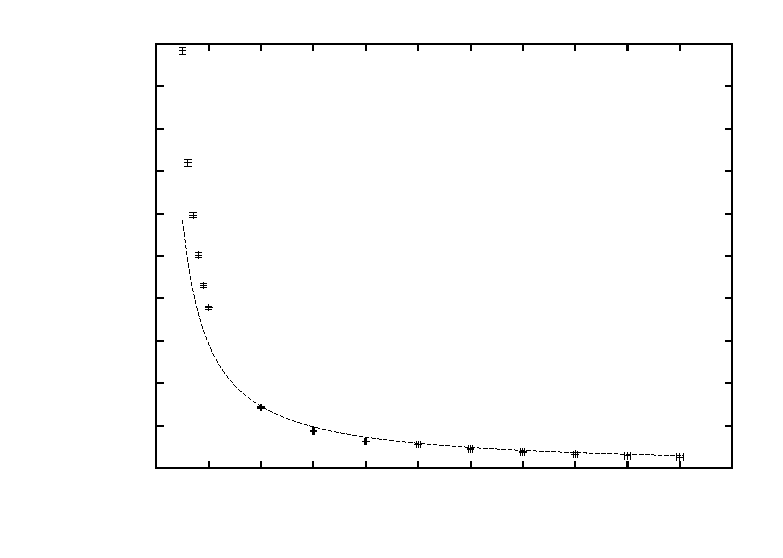
\includegraphics{g2}}%
    \gplfronttext
  \end{picture}%
\endgroup

    \caption{Graf závislosti frekvence na časové konstantě $\tau$}
    \label{g2}
    \end{figure}
    
    Dále jsem prověřoval závislost frekvenvce na napětí $U_0$. Odpor jsem ponechal na hodnotě 5 k$\Omega$ a začal s kapacitou 0.05 F. Hodnoty pro $\tau = 250$F$\Omega$
    jsou v tabulce \ref{TUk3a}. Při tomto nasta vení však nebyla příliš znatelná změná $U_{zh}$ a frekvence byla příliš vysoká. Proto jsem zvýšil kapacitu na 0.5 F 
    a výsladná časová konstanta je tedy $\tau = 2500$F$\Omega$. Naměřeně hodnoty jsou v tabulce \ref{TUk3b} a závislost je zobrazena na obrázku \ref{g3} a \ref{g4}.

    \begin{table}
    $$
    \begin{array}{|c|c|c|}
    \hline
    U_0/\mbox{V}&   f/\mbox{Hz}&    U_{zh}/\mbox{V} \\ \hline
    40.0\pm0.2& 4800\pm50&  11.0\pm0.2 \\ \hline
    50.1\pm0.2& 8100\pm80&  12.0\pm0.2 \\ \hline
    60.1\pm0.2& 11200\pm100&    13\pm0.2 \\ \hline
    70.0\pm0.2& 14100\pm100&    13\pm0.2 \\ \hline
    80.3\pm0.2& 17200\pm200&    13\pm0.2 \\ \hline
    \end{array}
    $$
    \caption{Závislost frekvence kmitů na $U_0$ pro $\tau=250$F$\Omega$}
    \label{TUk3a}
    \end{table}

    \begin{table}
    $$
    \begin{array}{|c|c|c|c|}
    \hline
    U_0/\mbox{V}&   f/\mbox{Hz}&    U_{zh}/\mbox{V}&    U_{BO}/\mbox{V} \\ \hline
    110.5\pm0.2&    2350\pm20&  12.0\pm0.2&   26\pm0.4 \\ \hline
    100.4\pm0.2&    2060\pm20&  12.0\pm0.2&   27\pm0.4 \\ \hline
    90.1\pm0.2&     1760\pm20&  11.5\pm0.2& 27\pm0.4 \\ \hline
    80.2\pm0.2&     1470\pm10&  11.5\pm0.2& 28\pm0.4 \\ \hline
    70.1\pm0.2&     1180\pm10&  11.0\pm0.2& 28\pm0.4 \\ \hline
    60.0\pm0.2&     888\pm9&    11.0\pm0.2& 28\pm0.4 \\ \hline
    50.3\pm0.2&     622\pm6&    10.5\pm0.2& 29\pm0.4 \\ \hline
    40.2\pm0.2&     343\pm3&    10.0\pm0.2& 30\pm0.5 \\ \hline
    \end{array}
    $$
    \caption{Závislost frekvence kmitů na $U_0$ pro $\tau=2500$F$\Omega$}
    \label{TUk3b}
    \end{table}
    
    \begin{figure}
    % GNUPLOT: LaTeX picture with Postscript
\begingroup
  \makeatletter
  \providecommand\color[2][]{%
    \GenericError{(gnuplot) \space\space\space\@spaces}{%
      Package color not loaded in conjunction with
      terminal option `colourtext'%
    }{See the gnuplot documentation for explanation.%
    }{Either use 'blacktext' in gnuplot or load the package
      color.sty in LaTeX.}%
    \renewcommand\color[2][]{}%
  }%
  \providecommand\includegraphics[2][]{%
    \GenericError{(gnuplot) \space\space\space\@spaces}{%
      Package graphicx or graphics not loaded%
    }{See the gnuplot documentation for explanation.%
    }{The gnuplot epslatex terminal needs graphicx.sty or graphics.sty.}%
    \renewcommand\includegraphics[2][]{}%
  }%
  \providecommand\rotatebox[2]{#2}%
  \@ifundefined{ifGPcolor}{%
    \newif\ifGPcolor
    \GPcolorfalse
  }{}%
  \@ifundefined{ifGPblacktext}{%
    \newif\ifGPblacktext
    \GPblacktexttrue
  }{}%
  % define a \g@addto@macro without @ in the name:
  \let\gplgaddtomacro\g@addto@macro
  % define empty templates for all commands taking text:
  \gdef\gplbacktext{}%
  \gdef\gplfronttext{}%
  \makeatother
  \ifGPblacktext
    % no textcolor at all
    \def\colorrgb#1{}%
    \def\colorgray#1{}%
  \else
    % gray or color?
    \ifGPcolor
      \def\colorrgb#1{\color[rgb]{#1}}%
      \def\colorgray#1{\color[gray]{#1}}%
      \expandafter\def\csname LTw\endcsname{\color{white}}%
      \expandafter\def\csname LTb\endcsname{\color{black}}%
      \expandafter\def\csname LTa\endcsname{\color{black}}%
      \expandafter\def\csname LT0\endcsname{\color[rgb]{1,0,0}}%
      \expandafter\def\csname LT1\endcsname{\color[rgb]{0,1,0}}%
      \expandafter\def\csname LT2\endcsname{\color[rgb]{0,0,1}}%
      \expandafter\def\csname LT3\endcsname{\color[rgb]{1,0,1}}%
      \expandafter\def\csname LT4\endcsname{\color[rgb]{0,1,1}}%
      \expandafter\def\csname LT5\endcsname{\color[rgb]{1,1,0}}%
      \expandafter\def\csname LT6\endcsname{\color[rgb]{0,0,0}}%
      \expandafter\def\csname LT7\endcsname{\color[rgb]{1,0.3,0}}%
      \expandafter\def\csname LT8\endcsname{\color[rgb]{0.5,0.5,0.5}}%
    \else
      % gray
      \def\colorrgb#1{\color{black}}%
      \def\colorgray#1{\color[gray]{#1}}%
      \expandafter\def\csname LTw\endcsname{\color{white}}%
      \expandafter\def\csname LTb\endcsname{\color{black}}%
      \expandafter\def\csname LTa\endcsname{\color{black}}%
      \expandafter\def\csname LT0\endcsname{\color{black}}%
      \expandafter\def\csname LT1\endcsname{\color{black}}%
      \expandafter\def\csname LT2\endcsname{\color{black}}%
      \expandafter\def\csname LT3\endcsname{\color{black}}%
      \expandafter\def\csname LT4\endcsname{\color{black}}%
      \expandafter\def\csname LT5\endcsname{\color{black}}%
      \expandafter\def\csname LT6\endcsname{\color{black}}%
      \expandafter\def\csname LT7\endcsname{\color{black}}%
      \expandafter\def\csname LT8\endcsname{\color{black}}%
    \fi
  \fi
  \setlength{\unitlength}{0.0500bp}%
  \begin{picture}(7200.00,5040.00)%
    \gplgaddtomacro\gplbacktext{%
      \csname LTb\endcsname%
      \put(1210,704){\makebox(0,0)[r]{\strut{} 0}}%
      \put(1210,1382){\makebox(0,0)[r]{\strut{} 500}}%
      \put(1210,2061){\makebox(0,0)[r]{\strut{} 1000}}%
      \put(1210,2739){\makebox(0,0)[r]{\strut{} 1500}}%
      \put(1210,3418){\makebox(0,0)[r]{\strut{} 2000}}%
      \put(1210,4096){\makebox(0,0)[r]{\strut{} 2500}}%
      \put(1210,4775){\makebox(0,0)[r]{\strut{} 3000}}%
      \put(1342,484){\makebox(0,0){\strut{} 30}}%
      \put(1956,484){\makebox(0,0){\strut{} 40}}%
      \put(2570,484){\makebox(0,0){\strut{} 50}}%
      \put(3184,484){\makebox(0,0){\strut{} 60}}%
      \put(3798,484){\makebox(0,0){\strut{} 70}}%
      \put(4413,484){\makebox(0,0){\strut{} 80}}%
      \put(5027,484){\makebox(0,0){\strut{} 90}}%
      \put(5641,484){\makebox(0,0){\strut{} 100}}%
      \put(6255,484){\makebox(0,0){\strut{} 110}}%
      \put(6869,484){\makebox(0,0){\strut{} 120}}%
      \put(308,2739){\rotatebox{-270}{\makebox(0,0){\strut{}$f$/Hz}}}%
      \put(4105,154){\makebox(0,0){\strut{}$U_0$/V}}%
    }%
    \gplgaddtomacro\gplfronttext{%
    }%
    \gplbacktext
    \put(0,0){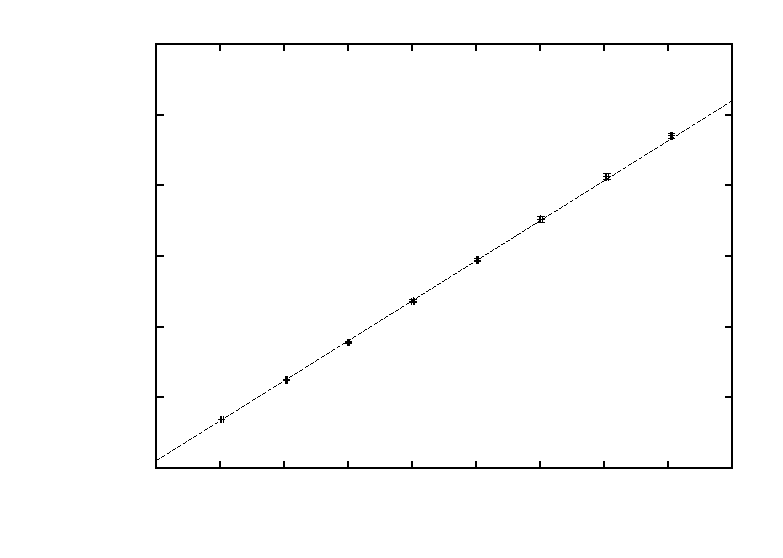
\includegraphics{g3}}%
    \gplfronttext
  \end{picture}%
\endgroup

    \caption{Graf závislosti frekvence na $U_0$}
    \label{g3}
    \end{figure}
    
    \begin{figure}
    % GNUPLOT: LaTeX picture with Postscript
\begingroup
  \makeatletter
  \providecommand\color[2][]{%
    \GenericError{(gnuplot) \space\space\space\@spaces}{%
      Package color not loaded in conjunction with
      terminal option `colourtext'%
    }{See the gnuplot documentation for explanation.%
    }{Either use 'blacktext' in gnuplot or load the package
      color.sty in LaTeX.}%
    \renewcommand\color[2][]{}%
  }%
  \providecommand\includegraphics[2][]{%
    \GenericError{(gnuplot) \space\space\space\@spaces}{%
      Package graphicx or graphics not loaded%
    }{See the gnuplot documentation for explanation.%
    }{The gnuplot epslatex terminal needs graphicx.sty or graphics.sty.}%
    \renewcommand\includegraphics[2][]{}%
  }%
  \providecommand\rotatebox[2]{#2}%
  \@ifundefined{ifGPcolor}{%
    \newif\ifGPcolor
    \GPcolorfalse
  }{}%
  \@ifundefined{ifGPblacktext}{%
    \newif\ifGPblacktext
    \GPblacktexttrue
  }{}%
  % define a \g@addto@macro without @ in the name:
  \let\gplgaddtomacro\g@addto@macro
  % define empty templates for all commands taking text:
  \gdef\gplbacktext{}%
  \gdef\gplfronttext{}%
  \makeatother
  \ifGPblacktext
    % no textcolor at all
    \def\colorrgb#1{}%
    \def\colorgray#1{}%
  \else
    % gray or color?
    \ifGPcolor
      \def\colorrgb#1{\color[rgb]{#1}}%
      \def\colorgray#1{\color[gray]{#1}}%
      \expandafter\def\csname LTw\endcsname{\color{white}}%
      \expandafter\def\csname LTb\endcsname{\color{black}}%
      \expandafter\def\csname LTa\endcsname{\color{black}}%
      \expandafter\def\csname LT0\endcsname{\color[rgb]{1,0,0}}%
      \expandafter\def\csname LT1\endcsname{\color[rgb]{0,1,0}}%
      \expandafter\def\csname LT2\endcsname{\color[rgb]{0,0,1}}%
      \expandafter\def\csname LT3\endcsname{\color[rgb]{1,0,1}}%
      \expandafter\def\csname LT4\endcsname{\color[rgb]{0,1,1}}%
      \expandafter\def\csname LT5\endcsname{\color[rgb]{1,1,0}}%
      \expandafter\def\csname LT6\endcsname{\color[rgb]{0,0,0}}%
      \expandafter\def\csname LT7\endcsname{\color[rgb]{1,0.3,0}}%
      \expandafter\def\csname LT8\endcsname{\color[rgb]{0.5,0.5,0.5}}%
    \else
      % gray
      \def\colorrgb#1{\color{black}}%
      \def\colorgray#1{\color[gray]{#1}}%
      \expandafter\def\csname LTw\endcsname{\color{white}}%
      \expandafter\def\csname LTb\endcsname{\color{black}}%
      \expandafter\def\csname LTa\endcsname{\color{black}}%
      \expandafter\def\csname LT0\endcsname{\color{black}}%
      \expandafter\def\csname LT1\endcsname{\color{black}}%
      \expandafter\def\csname LT2\endcsname{\color{black}}%
      \expandafter\def\csname LT3\endcsname{\color{black}}%
      \expandafter\def\csname LT4\endcsname{\color{black}}%
      \expandafter\def\csname LT5\endcsname{\color{black}}%
      \expandafter\def\csname LT6\endcsname{\color{black}}%
      \expandafter\def\csname LT7\endcsname{\color{black}}%
      \expandafter\def\csname LT8\endcsname{\color{black}}%
    \fi
  \fi
  \setlength{\unitlength}{0.0500bp}%
  \begin{picture}(7200.00,5040.00)%
    \gplgaddtomacro\gplbacktext{%
      \csname LTb\endcsname%
      \put(1210,704){\makebox(0,0)[r]{\strut{} 900}}%
      \put(1210,1383){\makebox(0,0)[r]{\strut{} 950}}%
      \put(1210,2061){\makebox(0,0)[r]{\strut{} 1000}}%
      \put(1210,2740){\makebox(0,0)[r]{\strut{} 1050}}%
      \put(1210,3418){\makebox(0,0)[r]{\strut{} 1100}}%
      \put(1210,4097){\makebox(0,0)[r]{\strut{} 1150}}%
      \put(1210,4775){\makebox(0,0)[r]{\strut{} 1200}}%
      \put(1342,484){\makebox(0,0){\strut{} 2}}%
      \put(2263,484){\makebox(0,0){\strut{} 3}}%
      \put(3184,484){\makebox(0,0){\strut{} 4}}%
      \put(4105,484){\makebox(0,0){\strut{} 5}}%
      \put(5027,484){\makebox(0,0){\strut{} 6}}%
      \put(5948,484){\makebox(0,0){\strut{} 7}}%
      \put(6869,484){\makebox(0,0){\strut{} 8}}%
      \put(308,2739){\rotatebox{-270}{\makebox(0,0){\strut{}$H$/Am$^{-1}$}}}%
      \put(4105,154){\makebox(0,0){\strut{}$x$/cm}}%
    }%
    \gplgaddtomacro\gplfronttext{%
      \csname LTb\endcsname%
      \put(5882,4602){\makebox(0,0)[r]{\strut{}teoretická}}%
      \csname LTb\endcsname%
      \put(5882,4382){\makebox(0,0)[r]{\strut{}fitovaná}}%
    }%
    \gplbacktext
    \put(0,0){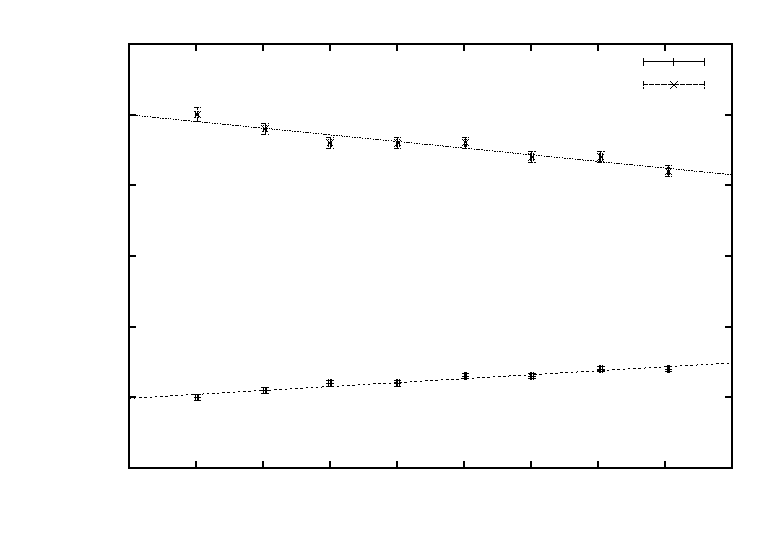
\includegraphics{g4}}%
    \gplfronttext
  \end{picture}%
\endgroup

    \caption{Graf závislosti $U_{BO}$ a $U_{zh}$ na $U_0$}
    \label{g4}
    \end{figure}

\section{Diskuze}
    Voltampérová charakteristiku diaku dobře odpovídá teoretickým předpokladům uvedeným v \cite{text}. Došlo 
    pouze k jemné odchylce při změně polarity. 

    Fit závislosti frekvence na $\tau$ má od teoretické odchylku okolo 5 \%. Největší chyba je především u nižších 
    hodnot $\tau$. To je podle mě způsobeno především nezapočítáním závislosti $U_{zh}$ a $U_{BO}$ na $U_0$, která 
    je vidět v úkolu 3. Také zajisté přispívá větší chyba způsobená vyššími hodnotami na čítači. Z hodnot frekvence 
    stanovenými jinými metodami je podle mě nejpřesnější hodnota vypočtená z periody změřené na osciloskopu, ač je třída 
    přesnosti osciloskopu relativně vysoká. Nejhorší je zajisté stupnice na generátoru, jejíž odchylka od hodnoty na čítači 
    dosahuje až 5 \%.

    Dle očekávání se velikost zhášecího napětí lineárně měnila se změnou $U_0$. Stejně tak tomu bylo i s $U_{BO}$. 
    Fitovaná křivka tak velmi dobře odpovídá teoretickým předpokladům.

\section{Závěr}
    Proměřil jem VA charakteristiku diaku. Výsledky jsou v tabulce \ref{TUk1} na na obrázku \ref{g1}. Zjistil jsem důležité 
    charakteristiky diaku, které jsou v rovnivích \ref{UBO1} - \ref{DU2}.

    Změřil jsem vývoj frekvence relaxačních kmitů v závislosti na změně $\tau$. Výsledky jsou v tabulce \ref{TUk2} a na obrázku \ref{g2}. 
    Použil jsem i jiné metody zjištění frekvence, kekiž výsledky jsou v tabulce \ref{TUk2b}.

    Z,ěřil jsem vývoj frekvence, $U_{BO}$ a $U_{zh}$ v závislosti na $U_0$. Výsledky jsou v tabulkách \ref{TUk3a}, \ref{TUk3b} a na obrázcích \ref{g3} a \ref{g4}. 

\begin{thebibliography}{5}
	\bibitem{text} \textbf{Studijní text na praktikum II} \\http://physics.mff.cuni.cz/vyuka/zfp/txt\_214.htm (28. 10. 2011)
    \bibitem{chyba} \emph{J. Englich}: \textbf{Zpracování výsldků fyzikálních měření} \\ LS 1999/2000
\end{thebibliography}



\end{document}
